\documentclass[11pt]{article}
\usepackage{charter}
\usepackage{graphicx}
\usepackage{hyperref}
\usepackage{mdframed}
\usepackage[margin=1in]{geometry}
\usepackage{amsmath,amssymb}

\hypersetup{
	colorlinks=true,
	linkcolor=blue,
	filecolor=magenta,
	urlcolor=cyan,
}

\begin{document}

%===================================================
% Title and Author Info
%===================================================
\begin{center}
{\Large\textsc{Relativistic Orbits}} \\
\vspace{10pt}
{\large \textbf{Mentor:} Alex Urban} \\
{\small LIGO Laboratory, California Institute of Technology \\
Pasadena, CA 91125, USA \\
\href{mailto:aurban@ligo.caltech.edu}{\texttt{aurban@ligo.caltech.edu}}}
\end{center}

%%%%%%%%%%%%%%%%%%%%%%%%%%%%%%%%%%%%%%%%%%%%%%%%%%%

\section*{Orbital Death Spirals and Hydrostatic Equilibrium}
\hspace{15pt} Suppose that a compact binary with masses $m_1$, $m_2$ is in a stable circular orbit. This time, we'll model its energy loss due to gravitational waves. Figure \ref{fig:binary_diagram} illustrates this system.

\vspace{20pt}

\begin{figure}[!h]
\begin{mdframed}
\centering
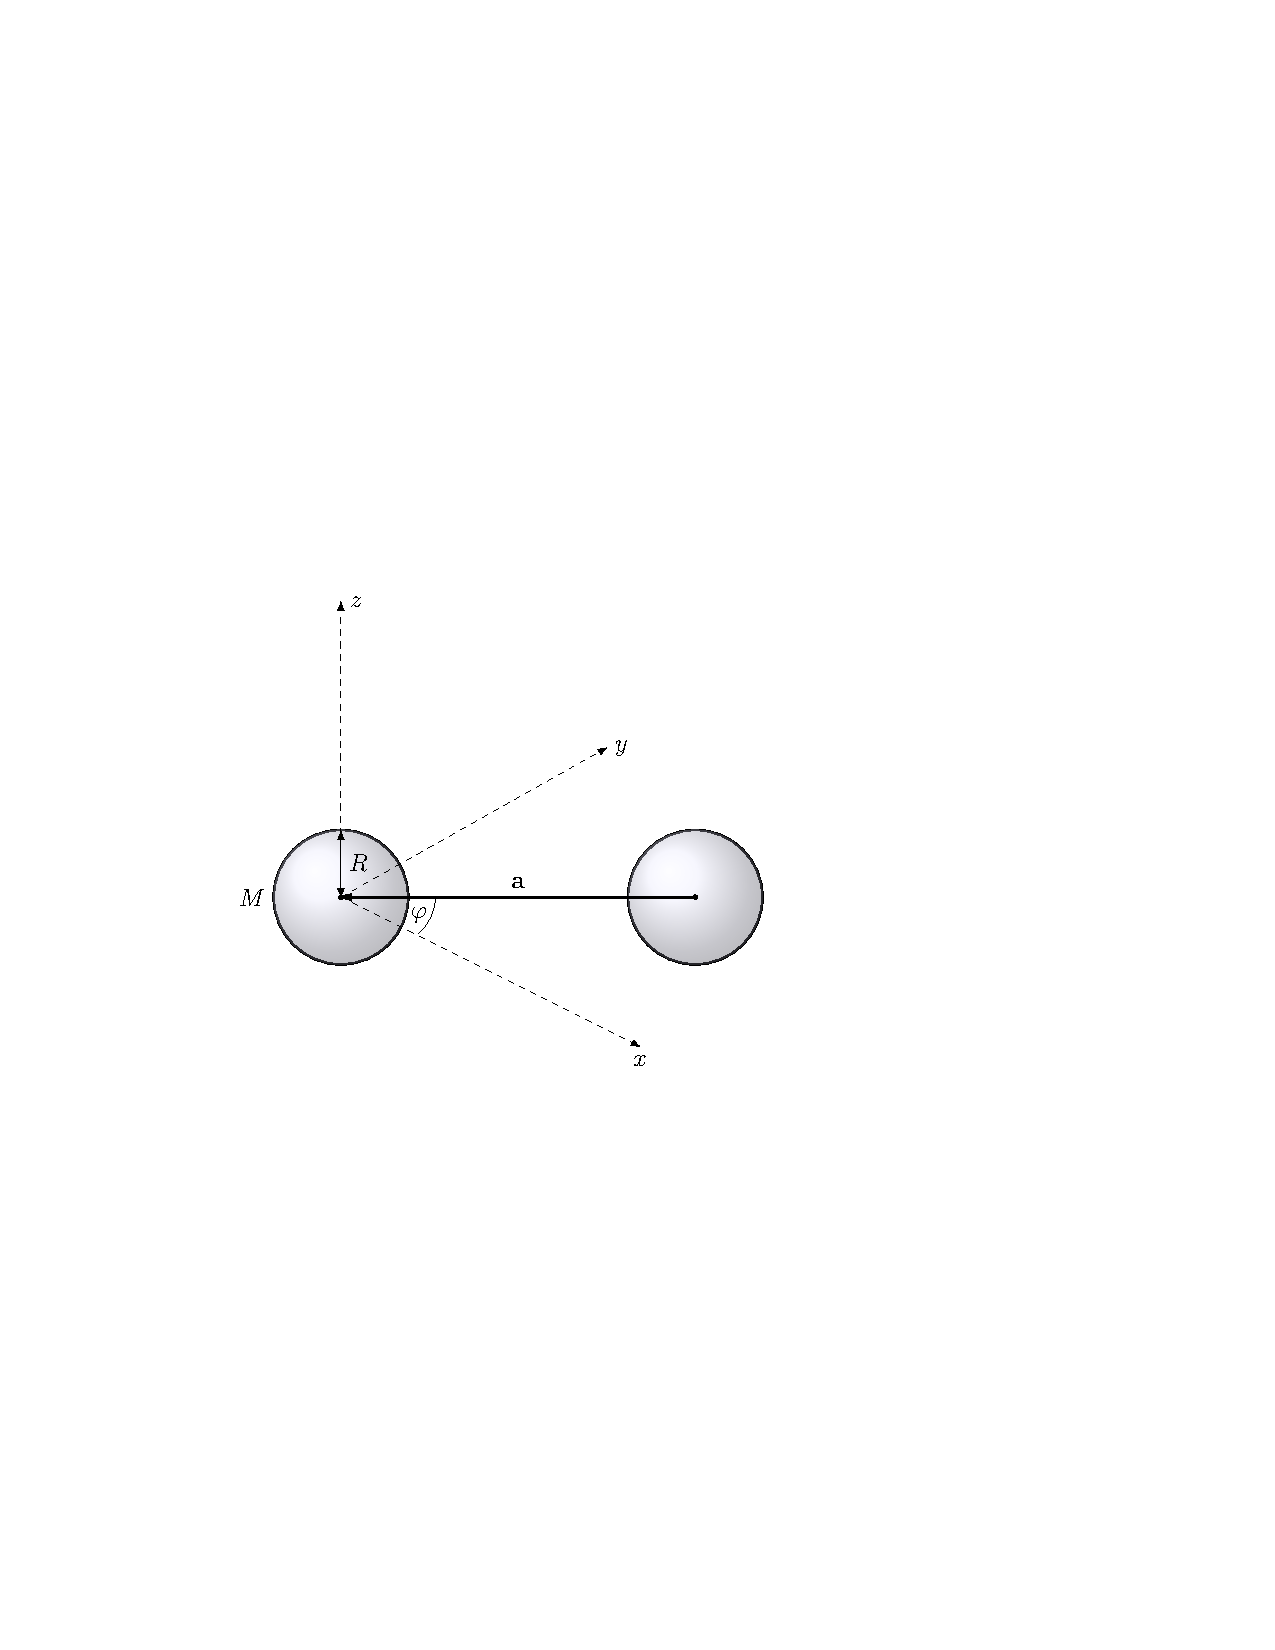
\includegraphics{relativistic_orbit/binary_diagram.pdf}
\caption{\label{fig:binary_diagram}Diagram of the neutron star binary in the center of mass frame, showing its orbital separation vector ($\mathbf{r}$) and the radius ($R$) and masses ($m_1$, $m_2$) of the individual neutron stars. The azimuthal angle $\varphi$ is also indicated.}
\end{mdframed}
\end{figure}

\vspace{10pt}

As we have seen, the orbiting binary is a simple example of a system with nonzero \textit{quadrupole moment} that changes over time. According to general relativity, this means the system will emit gravitational waves, which carry orbital energy away at a rate
\begin{equation}\label{eq:GW_luminosity}
-L_{\rm GW} = \frac{dE}{dt} = - \frac{32}{5} \frac{G^4}{c^5} \frac{\mu^2 M^3}{r^5}
\end{equation}
where $M = m_1 + m_2$ is the total mass and $\mu = m_1 m_2/(m_1 + m_2)$ is the reduced mass. (This is the observed ``luminosity'' in gravitational waves, which are emitted at twice the orbital frequency.)

\vspace{1000pt}

\begin{enumerate}

\item Using the fact that the gravitational binding energy of this system at a given time is
\[ E = - \frac{GM\mu}{2r}, \]
show that the orbital separation $r$ varies like
\begin{equation}\label{eq:drdt}
\frac{dr}{dt} = - \frac{64}{5} \frac{G^3}{c^5} \frac{\mu M^2}{r^3}.
\end{equation}
Can you solve this equation the old-fashioned way (\textit{i.e.} with pen and paper)?

\item How long does it take the orbit to evolve from a gravitational wave frequency of 20 Hz up to the ISCO frequency? Express this in terms of $\mu$ and $M$.

\item Numerically integrate equations \ref{eq:GW_luminosity} and \ref{eq:drdt} for a neutron star system with $m_1 = m_2 =$ 1.4 $M_{\odot}$. Plot the orbital separation, orbital velocity ($v/c$), kinetic, potential, and total energies, GW frequency, and the GW luminosity, all as a function of time. (You can start the integration from a separation of 300 km, and follow it all the way up to ISCO.)

\item Now, let's switch gears a bit and start building a model of very dense stellar material. To begin with, use Newtonian physics to try and show that an outward pressure on a spherical star will balance the inward pull of the star's gravity exactly when
\begin{equation}\label{eq:hydro}
\frac{dP}{dr} = - \frac{G}{r^2}\, \rho(r)\, m(r),
\end{equation}
where $\rho(r)$ is called the \textit{density profile} and
\begin{equation}\label{eq:mass}
\frac{dm}{dr} = 4 \pi r^2 \rho(r)
\end{equation}
is the mass contained in a thin spherical shell of radius $r$. (This condition, and the physical state it describes, is called \textit{hydrostatic equilibrium}.) What do $P(r)$ and $m(r)$ look like when the star is uniformly dense (so $\rho$ is a constant)?

\item In astrophysics, a \textit{polytrope} loosely refers to any object whose internal pressure and density are related by
\begin{equation}\label{eq:polytrope}
P = K \rho^{\gamma}
\end{equation}
where $K$ and $\gamma$ are constants. In particular, we can imagine, say, a gas of electrons that produce an outward pressure because no two of them can ever occupy the same quantum state (the Pauli exclusion principle). In this case, $\gamma =$ 5/3 and
\[ K = \frac{\hslash^2}{15\pi^2 m_e} \left( \frac{3\pi^2}{n m_N} \right)^{5/3} \]
where $m_e$ is the electron mass, $m_N$ the neutron mass, and $n$ the number of nucleons per electron. Try solving Eqs. \ref{eq:hydro} and \ref{eq:mass} numerically using this equation of state with $n=2$, which is a good model for a white dwarf star of total mass 1 $M_{\odot}$ and radius 10$^4$ km that's made mostly of neutral carbon.

\end{enumerate}

%%%%%%%%%%%%%%%%%%%%%%%%%%%%%%%%%%%%%%%%%%%%%%%%%%%

\section*{Things That Make You Go, ``Hmmm....''}

\begin{enumerate}

\item How does the rate of orbital decay (Eq. \ref{eq:drdt}) compare with the orbital velocity during your model of an inspiral?

\item Can you use this to justify the approximation we talked about last time, in which we can ignore radial acceleration when we account for forces during the inspiral?

\item What physics is the Newtonian condition for hydrostatic equilibrium (Eq. \ref{eq:hydro}) failing to capture?

\end{enumerate}

%%%%%%%%%%%%%%%%%%%%%%%%%%%%%%%%%%%%%%%%%%%%%%%%%%%
%%%%%%%%%%%%%%%%%%%%%%%%%%%%%%%%%%%%%%%%%%%%%%%%%%%
\vspace{1000pt}
%%%%%%%%%%%%%%%%%%%%%%%%%%%%%%%%%%%%%%%%%%%%%%%%%%%
%%%%%%%%%%%%%%%%%%%%%%%%%%%%%%%%%%%%%%%%%%%%%%%%%%%

\section*{Solution}

\begin{enumerate}

\item From the gravitational binding energy of the binary, we can take the time derivative and see that
\[ \frac{dE}{dt} = -\frac{d}{dt}\left(\frac{GM\mu}{2r}\right) = \frac{GM\mu}{2r^2} \frac{dr}{dt}. \]
From Eq. \ref{eq:GW_luminosity}, it's then clear that
\[ \frac{dr}{dt} = \frac{2r^2}{GM\mu} \frac{dE}{dt} = - \frac{64}{5} \frac{G^3}{c^5} \frac{\mu M^2}{r^3} \]
as we set out to show.

\hspace{15pt} Now, here's the cool part: isolating terms that vary with $r$ and terms that vary with $t$ on both sides, we wind up with the integrals
\[ 4 \int r^3 \, dr = - \frac{256}{5} \frac{G^3}{c^5} \mu M^2 \int dt. \]
But since there are two different variables on each side of the equation, these variables must depend on one another:
\[ r^4 - r_0^4 = - \frac{256}{5} \frac{G^3}{c^5} \mu M^2 \left(t - t_0\right) \]
where both $t_0$ and $r_0$ arise from constants of integration. Since they're not independent, we can lump them together into one constant called $t_c$ and rearrange:
\begin{equation}\label{eq:roft}
r(t) = \left[ r^4_{\rm ISCO} + \frac{256}{5}\,\frac{G^3}{c^5}\,\mu M^2 \left(t_c - t\right) \right]^{1/4}.
\end{equation}
In this case, we interpret $t_c$ as the time at which the binary reaches its innermost stable circular orbit and the objects ``coalesce,'' \textit{i.e.} $r(t_c) = r_{\rm ISCO}$. In LIGO jargon, this is the \textit{coalescence time}.

\item There is another way to interpret the integral in the previous problem. Namely, the time $\Delta t$ taken for the binary to evolve from any initial separation $r$ to any (smaller) separation $r_0 < r$ is
\[ \Delta t = \frac{5}{256} \frac{c^5}{G^3} \frac{1}{\mu M^2} \left(r^4 - r_0^4\right). \]
If $r_0 = 6GM/c^2$ is the ISCO radius and $r = [GM/(\pi f_{\rm GW})^2]^{1/3}$ is the separation at some GW frequency $f_{\rm GW} < f_{\rm ISCO}$, then
\[ \Delta t = \frac{5}{256} \frac{c^5}{G^3} \frac{1}{\mu M^2} \left[\left(\frac{GM}{(\pi f_{\rm GW})^2}\right)^{4/3} - \left(\frac{6GM}{c^2}\right)^4\right]. \]
If an equal-mass neutron star system with $m_1=m_2=$ 1.4 $M_{\odot}$ starts its evolution from $f_{\rm GW}=$ 20 Hz (or a separation of about 455 km), it will reach ISCO in $\Delta t \simeq$ 158 seconds (or about 2.5 minutes).

\hspace{15pt} This timescale is important because it's the amount of time a signal from compact binary merger remains in LIGO's sensitive frequency band, which currently starts around 20-30 Hz. The binary black hole signal GW 150914 was observed to last for around 0.2 seconds between 35 and 250 Hz with $m_1 \approx m_2 \approx$ 30 $M_{\odot}$, which is roughly in the same ballpark as our prediction that it should evolve from 35 Hz to $f_{\rm ISCO}$ in $\Delta t \simeq$ 0.175 seconds. But it's not exact. What do you think we're missing? And, just for kicks, what was the luminosity of this signal?

\item 

%%%%%%%%%%%%%%%%%%%%%%%%%%%%%%
\vspace{1000pt}

\item Let's picture a spherical shell of mass $\delta m$ and radius $r$ concentric with our hypothetical star, where the total mass contained inside is $m(r)$. Then the weight felt by this shell is
\[ \delta F = - \frac{G\,m(r)}{r^2}\,\delta m = -4\pi G \, \rho(r) \, m(r) \, \delta r \]
since $\delta m = 4\pi r^2 \rho(r) \, \delta r$ according to Eq. \ref{eq:mass}. In order to be in hydrostatic equilibrium, this inward gravitational pull must be balanced by an outward force
\[ \delta F = 4\pi r^2\,\delta P \]
where $\delta P$ is the pressure per unit area pushing outward against this shell. Setting the two equations equal and taking the limit as both $\delta r$ and $\delta P$ go to 0, we see that
\begin{equation}
\frac{dP}{dr} = - \frac{G}{r^2} \, \rho(r) \, m(r)
\end{equation}
which is just Eq. \ref{eq:hydro}, as we wanted to show.

\hspace{15pt} If the density profile $\rho(r) = \rho_* =$ const., then of course the mass
\[ m(r) = \frac{4}{3}\pi r^3 \rho_* \]
scales with the volume of the star -- that is, until we reach the radius $R_*$ of the star, at which point the density falls sharply to 0 and the mass plateus at $m_* = m(R_*)$. The radial pressure is easy to find:
\[ P(r\leq R_*) = -\frac{4}{3}\pi G\rho^2_* \int r\,dr = \frac{2}{3}\pi G\rho^2_*(R^2_* - r^2) \]
and $P(r>R_*) = 0$ outside of the star.

\hspace{15pt} Note that this model is pretty poor for a couple of reasons. First, physical materials don't remain uniformly dense inside of large bodies: the core of the Earth, for example, is crushed by the titanic weight of all the planet's layers sitting on top of it. Second, physical materials are also affected by thermodynamics, so they'll have an \textit{equation of state} relating $\rho$ and $P$, which we will of course explore in the next problem.

\item 

\end{enumerate}

\end{document}
